
\chapter[Tables in Python (2 of 3)]{\huge\selectfont{Tables in Python (2 of
3)}}

\index{row (of a \texttt{DataFrame})}
\index{row (of a table)}
\index{column (of a table)}

It's easy to get tripped up on Pandas' syntax for accessing the individual bits
of \texttt{DataFrame}s. First, let's talk about rows and columns, and then
we'll talk about the atomic elements (``cells'') themselves.

\section{Accessing individual rows and columns}

Suppose you have a \texttt{DataFrame} called \texttt{df}. Here's how you can
extract particular rows and columns:

\begin{compactitem}
\item \texttt{df.loc[}\textsl{i}\texttt{]} -- access the \textbf{row} with
\textbf{index} \textsl{i}
\item \texttt{df.iloc[}\textsl{n}\texttt{]} -- access \textbf{row} number
\textsl{n}
\item \texttt{df[}\textsl{c}\texttt{]} -- access \textbf{column} \textsl{c}
\end{compactitem}

\index{iloc@\texttt{.iloc} syntax (Pandas)}
\index{loc@\texttt{.loc} syntax (Pandas)}

The second of these is reminiscent of the \texttt{.iloc} syntax we learned for
\texttt{Series}es on p.~\pageref{iloc}. With it, we specify the \textit{number}
we want, rather than the index/key/label. That's not super common to do, but it
happens. More common is the first form: we specify the row we want by its
index.

The last one is tricky, because everyone (including me, several times a week,
it seems) assumes that just typing (say) ``\texttt{df['Bart']}'' would give you
\texttt{Bart}'s row. This is probably how it \textit{ought} to work, since
\texttt{Series}es worked that way. Alas, no: if you specify neither
\texttt{.loc} nor \texttt{.iloc}, you're asking for a \textit{column}, not a
row.

% WARNING: "bottom of" might not be correct if we change ch.16 text.

Yet another odd thing is how a single row is presented on the screen. Let's go
back to the \texttt{simpsons} data set (bottom of p.~\pageref{finalSimpsons}),
and access the \texttt{Bart} row the proper way (with \texttt{.loc}):

\begin{Verbatim}[fontsize=\small,samepage=true,frame=single,framesep=3mm]
print(simpsons.loc['Bart'])
\end{Verbatim}
\vspace{-.2in}

\begin{Verbatim}[fontsize=\small,samepage=true,frame=leftline,framesep=5mm,framerule=1mm]
species         human
age                10
gender              M
fave       skateboard
IQ                 90
hair             buzz
salary              0
Name: Bart, dtype: object
\end{Verbatim}

This bugs the heck out of me. Bart, like all other Simpsons, was a \textit{row}
in the original \texttt{DataFrame}, but here, it presents Bart's information
vertically instead of horizontally. I find it visually jarring. The reason
Pandas does it this way is that \textit{each row of a \texttt{DataFrame} is a
\texttt{Series}}, and the way Pandas displays \texttt{Series}es is vertically.
We'll deal somehow.

\index{double boxies@``double boxies''}

Btw, for any of the three options, you can provide a \textit{list} with
multiple things you want, instead of just one thing. You do so by using
\textit{double} boxies:

\begin{compactitem}
\item \texttt{df.loc[[}\textsl{i1,i2,i3,\dots}\texttt{]]} -- access the
row\textbf{s} with indices \textsl{i1, i2, i3,} \textit{etc.}
\item \texttt{df.iloc[[}\textsl{n1,n2,n3,\dots}\texttt{]]} -- access the row\textbf{s}
numbered \textsl{n1, n2, n3,} \textit{etc.}
\item \texttt{df[[}\textsl{c1,c2,c3,\dots}\texttt{]]} -- access the
column\textbf{s} names \textsl{c1, c2, c3,} \textit{etc.}
\end{compactitem}

\subsection{Examples}

To test your understanding of all of the above, confirm that you understand the
following examples:

\begin{Verbatim}[fontsize=\scriptsize,samepage=true,frame=single,framesep=3mm]
print(simpsons.iloc[3])
\end{Verbatim}
\vspace{-.2in}

\begin{Verbatim}[fontsize=\scriptsize,samepage=true,frame=leftline,framesep=5mm,framerule=1mm]
species        human
age                8
gender             F
fave       saxophone
IQ               200
hair           curly
salary             0
Name: Lisa, dtype: object
\end{Verbatim}

\medskip

\begin{Verbatim}[fontsize=\scriptsize,samepage=true,frame=single,framesep=3mm]
print(simpsons['age'])
\end{Verbatim}
\vspace{-.2in}

\begin{Verbatim}[fontsize=\scriptsize,samepage=true,frame=leftline,framesep=5mm,framerule=1mm]
name
Homer     36
Marge     34
Bart      10
Lisa       8
Maggie     1
SLH        4
Name: age, dtype: int64
\end{Verbatim}

\medskip
\begin{Verbatim}[fontsize=\scriptsize,samepage=true,frame=single,framesep=3mm]
print(simpsons.loc[['Lisa','Maggie','Bart']])
\end{Verbatim}
\vspace{-.2in}

\begin{Verbatim}[fontsize=\scriptsize,samepage=true,frame=leftline,framesep=5mm,framerule=1mm]
       species  age gender        fave     IQ   hair  salary
name                                                        
Lisa     human    8      F   saxophone  200.0  curly     0.0
Maggie   human    1      F    pacifier  100.0  curly     0.0
Bart     human   10      M  skateboard   90.0   buzz     0.0
\end{Verbatim}

\medskip
\begin{Verbatim}[fontsize=\scriptsize,samepage=true,frame=single,framesep=3mm]
print(simpsons.iloc[[1,3,4]])
\end{Verbatim}
\vspace{-.2in}

\begin{Verbatim}[fontsize=\scriptsize,samepage=true,frame=leftline,framesep=5mm,framerule=1mm]
       species  age gender            fave     IQ          hair  salary
name                                                                   
Marge    human   34      F  helping others  120.0  stacked tall     0.0
Lisa     human    8      F       saxophone  200.0         curly     0.0
Maggie   human    1      F        pacifier  100.0         curly     0.0
\end{Verbatim}

\medskip
\begin{Verbatim}[fontsize=\scriptsize,samepage=true,frame=single,framesep=3mm]
print(simpsons[['age','fave','IQ']])
\end{Verbatim}
\vspace{-.2in}

\begin{Verbatim}[fontsize=\scriptsize,samepage=true,frame=leftline,framesep=5mm,framerule=1mm]
        age            fave     IQ
name                              
Homer    36            beer   74.0
Marge    34  helping others  120.0
Bart     10      skateboard   90.0
Lisa      8       saxophone  200.0
Maggie    1        pacifier  100.0
SLH       4             NaN   30.0
\end{Verbatim}

Incidentally, you'll notice how the \texttt{name} values are treated
differently from all the other columns, since \texttt{name} is the
\texttt{DataFrame}'s index. For one thing, \texttt{name} \textit{always}
appears, even though it's not included among the columns we asked for. For
another, it's listed at the bottom of the single-row \texttt{Series} listings
rather than up with the other values in that row.

\section{Accessing individual elements}

I mentioned above the eternal truth that \textit{each row of a
\texttt{DataFrame} is a \texttt{Series}}. Once you grasp this, you'll realize
that you can access an individual ``cell'' of a \texttt{DataFrame} simply by
getting the row you want, and then getting the specific value from that. A
two-step process for doing this would be:

\begin{Verbatim}[fontsize=\small,samepage=true,frame=single,framesep=3mm]
lisas_row = simpsons.loc['Lisa']
lisas_iq = lisas_row['IQ']
print(lisas_iq)
\end{Verbatim}
\vspace{-.2in}

\begin{Verbatim}[fontsize=\small,samepage=true,frame=leftline,framesep=5mm,framerule=1mm]
200.0
\end{Verbatim}

But a shorter, one-stepper just combines these two operations on the same line:

\begin{Verbatim}[fontsize=\small,samepage=true,frame=single,framesep=3mm]
lisas_iq = simpsons.loc['Lisa']['IQ']
print(lisas_iq)
\end{Verbatim}
\vspace{-.2in}

\begin{Verbatim}[fontsize=\small,samepage=true,frame=leftline,framesep=5mm,framerule=1mm]
200.0
\end{Verbatim}

\section{Accessing a \texttt{DataFrame}'s metadata}

\index{metadata}
\index{index syntax@\texttt{.index} syntax (Pandas)}

We can get some meta-information about a \texttt{DataFrame} without even
looking at individual rows. If we want to know what the index values themselves
are, we use \texttt{.index}:

\begin{Verbatim}[fontsize=\small,samepage=true,frame=single,framesep=3mm]
print(simpsons.index)
\end{Verbatim}
\vspace{-.2in}

\begin{Verbatim}[fontsize=\small,samepage=true,frame=leftline,framesep=5mm,framerule=1mm]
Index(['Homer', 'Marge', 'Bart', 'Lisa', 'Maggie', 'SLH'],
    dtype='object', name='name')
\end{Verbatim}

That weird-looking output tells us several things. First, the index of this
\texttt{DataFrame} consists of \texttt{string}s (recall that's what
``\texttt{dtype='object'}'' means; see p.~\pageref{dtypeRules}.) Second, the
\textit{name} of the index column is, ironically, ``\texttt{name}''. (It could
be named anything at all, of course.) Third, the actual index values are
\texttt{Homer}, \texttt{Marge}, and all the rest.

\index{columns@\texttt{.columns} (Pandas)}

That's the index, or the ``row names,'' if you will. To get the column names,
we use \texttt{.columns}:

\begin{Verbatim}[fontsize=\small,samepage=true,frame=single,framesep=3mm]
print(simpsons.columns)
\end{Verbatim}
\vspace{-.2in}

\begin{Verbatim}[fontsize=\small,samepage=true,frame=leftline,framesep=5mm,framerule=1mm]
Index(['species', 'age', 'gender', 'fave', 'IQ', 'hair', 'salary'],
    dtype='object')
\end{Verbatim}

Interestingly, this too is an ``\texttt{Index}'' beast, also comprised of
\texttt{string}s. Pandas treats both ``axes'' of a \texttt{DataFrame}
similarly, in that both of them are the same type of thing (an
``\texttt{Index}''). Notice that \texttt{name} is not present in the column
names list, because as the \texttt{DataFrame}'s index it's a different sort of
thing.

\index{len@\texttt{len()}}

How many rows does a \texttt{DataFrame} have? This is answerable by using the
\texttt{len()} function again:

\begin{Verbatim}[fontsize=\small,samepage=true,frame=single,framesep=3mm]
print(len(simpsons))
\end{Verbatim}
\vspace{-.2in}

\begin{Verbatim}[fontsize=\small,samepage=true,frame=leftline,framesep=5mm,framerule=1mm]
6
\end{Verbatim}

This is our third use of the word \texttt{len()}: it can be used to find the
number of characters in a \texttt{string}, the number of key/value pairs of a
\texttt{Series}, and (here) the number of rows of a \texttt{DataFrame}.

\index{shape@\texttt{.shape} (Pandas)}
Finally, we often want to get a quick sense of how large a \texttt{DataFrame}
is, both in terms of rows and columns. The \texttt{.shape} syntax is handy
here:

\begin{samepage}
\begin{Verbatim}[fontsize=\small,samepage=true,frame=single,framesep=3mm]
print(simpsons.shape)
\end{Verbatim}
\vspace{-.2in}

\begin{Verbatim}[fontsize=\small,samepage=true,frame=leftline,framesep=5mm,framerule=1mm]
(6, 7)
\end{Verbatim}
\end{samepage}

This tells us that \texttt{simpsons} has six rows and seven columns. As I
mentioned previously (p.~\pageref{tallAndSkinny}) this is definitely not the
typical case: most \texttt{DataFrames} will have many more rows (thousands or
even millions) than columns (at most, dozens).

\section{Sorting \texttt{DataFrames}s}
\index{sorting@sorting (\texttt{DataFrame}s)}

Sorting a \texttt{DataFrame} is largely like sorting a \texttt{Series}, except
we have more choices: instead of just the keys and the values, we have the
index and potentially \textit{many} different columns.

\index{sort\_index@\texttt{.sort\_index()} method (Pandas)}
The \texttt{.sort\_index()} method works just like it did for
\texttt{Series}es:

\begin{samepage}
\begin{Verbatim}[fontsize=\small,samepage=true,frame=single,framesep=3mm]
print(simpsons.sort_index())
\end{Verbatim}
\vspace{-.2in}

\begin{Verbatim}[fontsize=\small,samepage=true,frame=leftline,framesep=5mm,framerule=1mm]
       species  age gender            fave     IQ          hair   salary
name                                                                    
Bart     human   10      M      skateboard   90.0          buzz      0.0
Homer    human   36      M            beer   74.0          none  52000.0
Lisa     human    8      F       saxophone  200.0         curly      0.0
Maggie   human    1      F        pacifier  100.0         curly      0.0
Marge    human   34      F  helping others  120.0  stacked tall      0.0
SLH        dog    4      M             NaN   30.0        shaggy      0.0
\end{Verbatim}
\end{samepage}

The result is rows sorted alphabetically by name. And I hate to keep repeating
myself, but remember that \texttt{.sort\_index()} returns a modified copy,
unless you pass the \texttt{inplace=True} argument. The
\texttt{ascending=False} argument is also allowed, and will sort by the index
highest-to-lowest instead of lowest-to-highest.

\index{sort\_values@\texttt{.sort\_values()} method (Pandas)}
To sort by one of the columns, we call \texttt{.sort\_values()} and pass it the
column name:

\begin{Verbatim}[fontsize=\small,samepage=true,frame=single,framesep=3mm]
print(simpsons.sort_index('IQ')
\end{Verbatim}
\vspace{-.2in}

\begin{Verbatim}[fontsize=\small,samepage=true,frame=leftline,framesep=5mm,framerule=1mm]
       species  age gender            fave     IQ          hair   salary
name                                                                    
SLH        dog    4      M             NaN   30.0        shaggy      0.0
Homer    human   36      M            beer   74.0          none  52000.0
Bart     human   10      M      skateboard   90.0          buzz      0.0
Maggie   human    1      F        pacifier  100.0         curly      0.0
Marge    human   34      F  helping others  120.0  stacked tall      0.0
Lisa     human    8      F       saxophone  200.0         curly      0.0
\end{Verbatim}

\index{tie-breaker}

Sometimes we want to include more than one column in the sort. Why? As a
tie-breaker. Consider sorting a roster for a student club, which has
\texttt{first\_name} and \texttt{last\_name} columns, among other things. We
might want to sort the list alphabetically by last name, but for students with
the same last name, we should go to the first name as a tie-breaker (so that
\texttt{Angela Smith} shows up after \texttt{Velma Patterson} but before
\texttt{Brad Smith}).

To do this, we pass a list of columns, instead of a single column:

\begin{samepage}
\begin{Verbatim}[fontsize=\small,samepage=true,frame=single,framesep=3mm]
print(simpsons.sort_values(['gender','hair','IQ']))
\end{Verbatim}
\vspace{-.2in}

\begin{Verbatim}[fontsize=\small,samepage=true,frame=leftline,framesep=5mm,framerule=1mm]
       species  age gender            fave     IQ          hair   salary
name                                                                    
Maggie   human    1      F        pacifier  100.0         curly      0.0
Lisa     human    8      F       saxophone  200.0         curly      0.0
Marge    human   34      F  helping others  120.0  stacked tall      0.0
Bart     human   10      M      skateboard   90.0          buzz      0.0
Homer    human   36      M            beer   74.0          none  52000.0
SLH        dog    4      M             NaN   30.0        shaggy      0.0
\end{Verbatim}
\end{samepage}

Here, we said ``sort the rows alphabetically by \texttt{gender}. For rows with
the same \texttt{gender}, use \texttt{hair} as a tie-breaker. And for rows with
the same \texttt{gender} \textit{and} the same \texttt{hair}, use \texttt{IQ}
as a second tie-breaker.'' Glance at that output and convince yourself that
it's correct.

We control the ``ascendingness'' of the multi-column sort by specifying a list
of \textit{each} \texttt{ascending} value, one for each column we're sorting
by. Consider this:

\begin{samepage}
\begin{Verbatim}[fontsize=\small,samepage=true,frame=single,framesep=3mm]
print(simpsons.sort_values(['gender','hair','IQ'],
    ascending=[False,True,False]))
\end{Verbatim}
\vspace{-.2in}

\begin{Verbatim}[fontsize=\small,samepage=true,frame=leftline,framesep=5mm,framerule=1mm]
       species  age gender            fave     IQ          hair   salary
name                                                                    
Bart     human   10      M      skateboard   90.0          buzz      0.0
Homer    human   36      M            beer   74.0          none  52000.0
SLH        dog    4      M             NaN   30.0        shaggy      0.0
Lisa     human    8      F       saxophone  200.0         curly      0.0
Maggie   human    1      F        pacifier  100.0         curly      0.0
Marge    human   34      F  helping others  120.0  stacked tall      0.0
\end{Verbatim}
\end{samepage}

Now we're saying ``sort \textit{reverse} alphabetically by \texttt{gender},
breaking ties by comparing \texttt{hair} alphabetically, and breaking further
ties by \texttt{reverse} sorted order by IQ.''

Oh, and the \texttt{inplace=True} argument works for all these examples as
well.

\section{Summary statistics for \texttt{DataFrame}s}

\index{summary statistics}

Summary statistics like the mean, median, minimum/maximum, and the like, can of
course all be computed on individual columns of a \texttt{DataFrame}, because
each column is a \texttt{Series}:

\index{median}

\begin{samepage}
\begin{Verbatim}[fontsize=\small,samepage=true,frame=single,framesep=3mm]
print(simpsons['IQ'].median())
\end{Verbatim}
\vspace{-.2in}

\begin{Verbatim}[fontsize=\small,samepage=true,frame=leftline,framesep=5mm,framerule=1mm]
95.0
\end{Verbatim}
\end{samepage}

\begin{samepage}
\begin{Verbatim}[fontsize=\small,samepage=true,frame=single,framesep=3mm]
print(simpsons['salary'].sum())
\end{Verbatim}
\vspace{-.2in}

\index{sum method@\texttt{.sum()} method (Pandas)}
\begin{Verbatim}[fontsize=\small,samepage=true,frame=leftline,framesep=5mm,framerule=1mm]
52000.0
\end{Verbatim}
\end{samepage}

\index{mean method@\texttt{.mean()} method (Pandas)}
You can also, believe it or not, compute the sum/mean/max/etc on the entire
\texttt{DataFrame}. This computes it on every column individually:

\begin{samepage}
\begin{Verbatim}[fontsize=\small,samepage=true,frame=single,framesep=3mm]
print(simpsons.mean())
\end{Verbatim}
\vspace{-.2in}

\begin{Verbatim}[fontsize=\small,samepage=true,frame=leftline,framesep=5mm,framerule=1mm]
age         15.500000
IQ         102.333333
salary    8666.666667
dtype: float64
\end{Verbatim}
\end{samepage}


Pandas left out the non-numeric columns (\texttt{species}, \texttt{gender},
\textit{etc.}) and computed the mean of each of the others, giving us a
\texttt{Series} containing their values.

\index{describe method@\texttt{.describe()} method (Pandas)}

Finally, I often find the \texttt{.describe()} method useful:

\begin{samepage}
\begin{Verbatim}[fontsize=\small,samepage=true,frame=single,framesep=3mm]
print(simpsons.describe())
\end{Verbatim}
\vspace{-.2in}

\begin{Verbatim}[fontsize=\small,samepage=true,frame=leftline,framesep=5mm,framerule=1mm]
count   6.000000    6.000000      6.000000
mean   15.500000  102.333333   8666.666667
std    15.436969   56.645094  21228.911104
min     1.000000   30.000000      0.000000
25%     5.000000   78.000000      0.000000
50%     9.000000   95.000000      0.000000
75%    28.000000  115.000000      0.000000
max    36.000000  200.000000  52000.000000
\end{Verbatim}
\end{samepage}

\index{quartile}
\index{standard deviation}

Neat! We get the number of values, the mean, the standard deviation, and all
the quartiles for each of the numeric columns. Lots of dashboard information at
a glance!

% recoding with vectorized operators (and adding new column)


%\section{Vectorized arithmetic operators}
%
%As with NumPy \texttt{ndarrays}, you can apply arithmetic operators like
%\texttt{+} and \texttt{*} to entire \texttt{Series}es at a time, which is not
%only easy code to write but also runs blazing fast. But the Pandas
%\texttt{Series} is even smarter than that.
%
%\begin{figure}[ht]
%\centering
%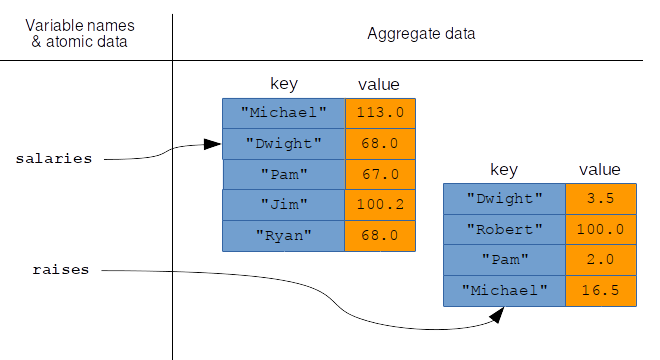
\includegraphics[width=0.9\textwidth]{vectorizedPandas.png}
%\caption{Two \texttt{Series}es in memory}
%\label{fig:vectorizedPandas}
%\end{figure}
%
%Consider the memory picture in Figure~\ref{fig:vectorizedPandas}. Here we have
%two \texttt{Series}es, one pointed to by a \texttt{salaries} variable and the
%other by \texttt{raises}, which are of different sizes and which have
%overlapping, but not identical, sets of keys. What do you suppose Pandas would
%do if we executed this code?
%
%\begin{Verbatim}[fontsize=\small,samepage=true,frame=single,framesep=3mm]
%new_salaries = salaries + raises
%\end{Verbatim}
%
%The answer, happily, is the smartest possible thing it could do. Pandas gets
%neither confused nor stifled by the fact that the keys are in different orders
%in the two \texttt{Series}es, and instead it does what you surely want:
%add corresponding elements, with matching keys, and produce a new
%\texttt{Series} with all of those sums.
%
%\begin{figure}[ht]
%\centering
%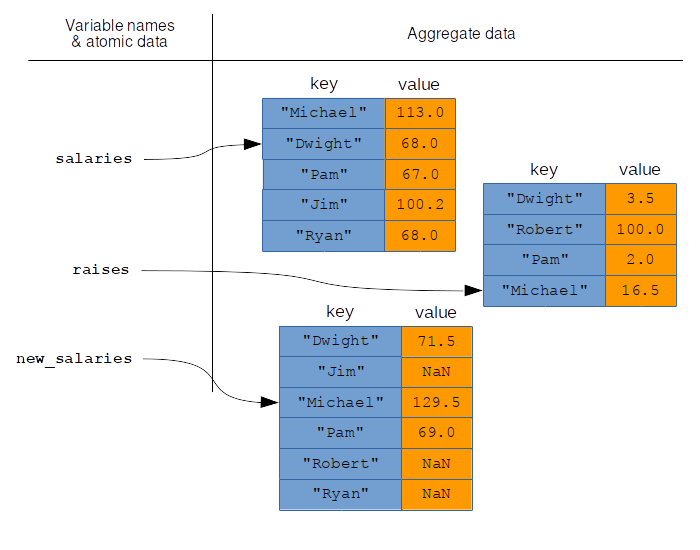
\includegraphics[width=0.8\textwidth]{vectorizedPandas2.png}
%\caption{The result of \texttt{+}'ing two \texttt{Series}es that don't have all the same keys.}
%\label{fig:vectorizedPandas2}
%\end{figure}
%
%The actual result in this case is in Figure~\ref{fig:vectorizedPandas2}, and
%the output is here:
%
%% salaries = pd.Series([113,68,67,100.2,68],
%%   index=['Michael','Dwight','Pam','Jim','Ryan'])
%% raises = pd.Series([3.5,100,2,16.5],
%%   index=['Dwight','Robert','Pam','Michael'])
%
%\begin{Verbatim}[fontsize=\small,samepage=true,frame=single,framesep=3mm]
%new_salaries = salaries + raises
%print(new_salaries)
%\end{Verbatim}
%
%\begin{Verbatim}[fontsize=\small,samepage=true,frame=leftline,framesep=5mm,framerule=1mm]
%Dwight      71.5
%Jim          NaN
%Michael    129.5
%Pam         69.0
%Robert       NaN
%Ryan         NaN
%dtype: float64
%\end{Verbatim}
%
%\index{nan@\texttt{NaN} (``not a number'')}
%\index{missing value}
%
%Convince yourself that \texttt{Dwight}'s \$68,000 salary got added to his
%\$3,500 raise, and that \texttt{Michael}'s \$113,000 was added to \$16,500,
%\textit{etc.}
%
%\label{NaN}
%
%Don't get freaked out by those \texttt{NaN} entries just yet. The special value
%``\textbf{NaN}'' stands for ``\textbf{not a number},'' and basically means that
%Pandas has to throw up its hands in that case. And with good cause.
%\texttt{Jim} has a current salary of \$100,200 in the first \texttt{Series},
%but has no value at all in the second one (no raise for Jim this year? Haven't
%decided what his raise will be yet? Something else?) and so Pandas shrugs and
%says ``dunno.'' We say that the \texttt{Jim} entry in the
%\texttt{new\_salaries} \texttt{Series} is a \textbf{missing value}. The same is
%true for \texttt{Robert} and \texttt{Ryan}, each of whom was present in only
%one of the two operands.
%
%Now I know what you're thinking: ``can't Pandas just assume the salary and/or
%raise is 0 if there's a missing one?'' The answer is that yes it can, but it
%won't do so unless you give the go-ahead. Pandas is being cautious here, and
%doesn't want to introduce errors into your data stream by false assumptions.
%(Maybe in your company, for instance, there's a default entry-level salary that
%every employee receives who's unspecified in the \texttt{salary}
%\texttt{Series}. Or maybe the yearly raise is always assumed to be a flat 2.5\%
%cost-of-living raise unless explicitly specified.)
%
%\index{add@\texttt{add()} function (Pandas)}
%\index{sub@\texttt{sub()} function (Pandas)}
%\index{mul@\texttt{mul()} function (Pandas)}
%\index{div@\texttt{div()} function (Pandas)}
%
%If we do want Pandas to assume a certain default value, we have to change
%tactics a bit and go with the \texttt{add()} function (or \texttt{sub()},
%\texttt{mul()}, or \texttt{div()}):
%
%\begin{Verbatim}[fontsize=\small,samepage=true,frame=single]
%new_salaries = pd.Series.add(salaries, raises, fill_value=0)
%print(new_salaries)
%\end{Verbatim}
%
%\begin{Verbatim}[fontsize=\small,samepage=true,frame=leftline,framesep=5mm,framerule=1mm]
%Dwight      71.5
%Jim        100.2
%Michael    129.5
%Pam         69.0
%Robert     100.0
%Ryan        68.0
%dtype: float64
%\end{Verbatim}
%
%The \texttt{fill\_value} argument is the important one here: it specifies what
%default value to use if one of the addends is missing a key from the other. Now
%the result is as in Figure~\ref{fig:vectorizedPandas3}. You can, of course,
%choose a \texttt{fill\_value} other than zero, if you wish.
%
%\begin{figure}[ht]
%\centering
%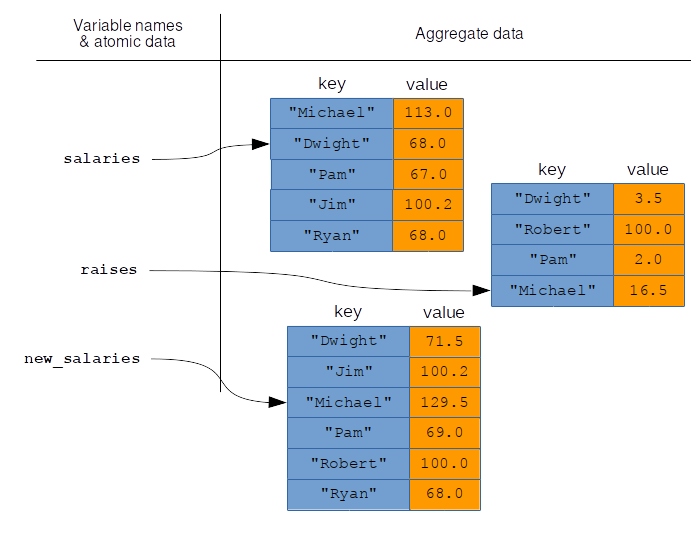
\includegraphics[width=0.8\textwidth]{vectorizedPandas3.png}
%\caption{Using \texttt{add()} instead, and passing a \texttt{fill\_value}.}
%\label{fig:vectorizedPandas3}
%\end{figure}
%
%As with NumPy arrays, we can add (or subtract, or multiply, ...) a single
%atomic value to a series as well:
%
%\begin{Verbatim}[fontsize=\small,samepage=true,frame=single,framesep=3mm]
%cost_of_living_increase = salaries * .025
%print(cost_of_living_increase)
%\end{Verbatim}
%
%\begin{Verbatim}[fontsize=\small,samepage=true,frame=leftline,framesep=5mm,framerule=1mm]
%Michael    2.825
%Dwight     1.700
%Pam        1.675
%Jim        2.505
%Ryan       1.700
%dtype: float64
%\end{Verbatim}
%
%\begin{Verbatim}[fontsize=\small,samepage=true,frame=single,framesep=3mm]
%salaries = salaries + cost_of_living_increase
%print(salaries)
%\end{Verbatim}
%
%\begin{Verbatim}[fontsize=\small,samepage=true,frame=leftline,framesep=5mm,framerule=1mm]
%Michael    115.825
%Dwight      69.700
%Pam         68.675
%Jim        102.705
%Ryan        69.700
%dtype: float64
%\end{Verbatim}
%
%It can sometimes be useful to do string concatenation as well, for instance if
%we had employee first names and last names in two \texttt{Series}es with their
%employee ID as the index:
%
%\begin{Verbatim}[fontsize=\small,samepage=true,frame=single,framesep=3mm]
%firsts = pd.Series(['Hannibal', 'Clarice', 'Multiple', 'Buffalo'],
%    index=[666, 1993, 47, 988])
%lasts = pd.Series(['Starling', 'Crawford', 'Lecter', 'Bill', 'Miggs'],
%    index=[1993, 1650, 666, 988, 47])
%print(firsts + " " + lasts)
%\end{Verbatim}
%
%\begin{Verbatim}[fontsize=\small,samepage=true,frame=leftline,framesep=5mm,framerule=1mm]
%47        Multiple Miggs
%666      Hannibal Lecter
%988         Buffalo Bill
%1650                 NaN
%1993    Clarice Starling
%dtype: object
%\end{Verbatim}
%
%\section{Copying \texttt{Series}es}
%
%\index{copying@copying (\texttt{Series}es)}
%The rules for copying (or not copying) \texttt{Series}es are exactly the same
%as for NumPy arrays (see Section~\ref{copyingNotCopyingArrays} on
%p.~\pageref{copyingNotCopyingArrays}). If you merely assign one \texttt{Series}
%object to another variable, the two variables will be pointing to the
%\textit{same} \texttt{Series} in memory, which means that changes to one will
%be reflected in the other. Calling the \texttt{.copy()} method, however,
%creates an entirely new \texttt{Series} in memory.
%
%Make sure you understand the following output to confirm your understanding of
%this:
%
%\index{Buffy the Vampire Slayer@\textit{Buffy the Vampire Slayer}}
%
%\begin{Verbatim}[fontsize=\scriptsize,samepage=true,frame=single,framesep=3mm]
%slayers = pd.Series([120, 72, 200], index=['Buffy','Xander','Willow'])
%anti_vamps = slayers
%good_guys = slayers.copy()
%anti_vamps['Rubert'] = 150
%print(slayers)
%\end{Verbatim}
%\vspace{-.3in}
%
%\begin{Verbatim}[fontsize=\scriptsize,samepage=true,frame=leftline,framesep=5mm,framerule=1mm]
%Buffy     120
%Xander     72
%Willow    200
%Rubert    150
%dtype: int64
%\end{Verbatim}
%
%\begin{Verbatim}[fontsize=\scriptsize,samepage=true,frame=single,framesep=3mm]
%print(anti_vamps)
%\end{Verbatim}
%\vspace{-.3in}
%
%\begin{Verbatim}[fontsize=\scriptsize,samepage=true,frame=leftline,framesep=5mm,framerule=1mm]
%Buffy     120
%Xander     72
%Willow    200
%Rubert    150
%dtype: int64
%\end{Verbatim}
%
%\begin{Verbatim}[fontsize=\scriptsize,samepage=true,frame=single,framesep=3mm]
%print(good_guys)
%\end{Verbatim}
%\vspace{-.3in}
%
%\begin{Verbatim}[fontsize=\scriptsize,samepage=true,frame=leftline,framesep=5mm,framerule=1mm]
%Buffy     120
%Xander     72
%Willow    200
%dtype: int64
%\end{Verbatim}
%
%(The numbers here are approximate IQs; don't mean to be a hater.)
%
%
%\section{Sorting \texttt{Series}es}
%\index{sorting@sorting (\texttt{Series}es)}
%\index{sort\_values@\texttt{.sort\_values()} method (Pandas)}
%\index{sort\_index@\texttt{.sort\_index()} method (Pandas)}
%
%Sorting is slightly more complex than for arrays, since there are two things we
%might want to sort by: the \texttt{Series}' index, or the values themselves.
%Correspondingly, there are two methods: \texttt{.sort\_index()} and
%\texttt{.sort\_values()}:
%
%\begin{Verbatim}[fontsize=\small,samepage=true,frame=single,framesep=3mm]
%print(anti_vamps.sort_index())
%\end{Verbatim}
%\vspace{-.3in}
%
%\begin{Verbatim}[fontsize=\small,samepage=true,frame=leftline,framesep=5mm,framerule=1mm]
%Buffy     120
%Rubert    150
%Willow    200
%Xander     72
%dtype: int64
%\end{Verbatim}
%
%\begin{Verbatim}[fontsize=\small,samepage=true,frame=single,framesep=3mm]
%print(anti_vamps.sort_values())
%\end{Verbatim}
%\vspace{-.3in}
%
%\begin{Verbatim}[fontsize=\small,samepage=true,frame=leftline,framesep=5mm,framerule=1mm]
%Xander     72
%Buffy     120
%Rubert    150
%Willow    200
%dtype: int64
%\end{Verbatim}
%
%\index{in place@``in place''}
%Like NumPy's \texttt{np.sort()} function (but unlike its \texttt{.sort()}
%method; refer back to Section~\ref{sortingArrays} on p.~\pageref{sortingArrays}
%for details), neither of these methods actually sort the \texttt{Series} in
%place; instead, they return sorted copies. However, they can be made to, by
%including ``\texttt{inplace=True}'' as an argument:
%
%\begin{Verbatim}[fontsize=\small,samepage=true,frame=single,framesep=3mm]
%heroes_dumb_to_smart = anti_vamps.sort_values()
%print(heroes_dumb_to_smart)
%\end{Verbatim}
%\vspace{-.3in}
%
%\begin{Verbatim}[fontsize=\small,samepage=true,frame=leftline,framesep=5mm,framerule=1mm]
%Xander     72
%Buffy     120
%Rubert    150
%Willow    200
%dtype: int64
%\end{Verbatim}
%
%\begin{Verbatim}[fontsize=\small,samepage=true,frame=single,framesep=3mm]
%print(anti_vamps)
%\end{Verbatim}
%\vspace{-.3in}
%
%\begin{Verbatim}[fontsize=\small,samepage=true,frame=leftline,framesep=5mm,framerule=1mm]
%Buffy     120
%Xander     72
%Willow    200
%Rubert    150
%dtype: int64
%\end{Verbatim}
%
%\begin{Verbatim}[fontsize=\small,samepage=true,frame=single,framesep=3mm]
%anti_vamps.sort_values(inplace=True)
%print(anti_vamps)
%\end{Verbatim}
%\vspace{-.3in}
%
%\begin{Verbatim}[fontsize=\small,samepage=true,frame=leftline,framesep=5mm,framerule=1mm]
%Xander     72
%Buffy     120
%Rubert    150
%Willow    200
%dtype: int64
%\end{Verbatim}
%
%Another useful feature of both \texttt{.sort\_X} methods is the ability to
%\textit{reverse} sort. By adding ``\texttt{ascending=False}'' as an argument
%(with or without also including the ``\texttt{inplace=True}'' argument; they
%are combinable with a comma) you produce the reverse order:
%
%\begin{Verbatim}[fontsize=\small,samepage=true,frame=single,framesep=3mm]
%heroes_smart_to_dumb = anti_vamps.sort_values(ascending=False)
%print(heroes_smart_to_dumb)
%\end{Verbatim}
%\vspace{-.3in}
%
%\begin{Verbatim}[fontsize=\small,samepage=true,frame=leftline,framesep=5mm,framerule=1mm]
%Willow    200
%Rubert    150
%Buffy     120
%Xander     72
%dtype: int64
%\end{Verbatim}
%
%\begin{Verbatim}[fontsize=\small,samepage=true,frame=single,framesep=3mm]
%anti_vamps.sort_index(inplace=True, ascending=False)
%print(anti_vamps)
%\end{Verbatim}
%\vspace{-.3in}
%
%\begin{Verbatim}[fontsize=\small,samepage=true,frame=leftline,framesep=5mm,framerule=1mm]
%Xander     72
%Willow    200
%Rubert    150
%Buffy     120
%dtype: int64
%\end{Verbatim}
%
%\section{Concatenating and combining}
%
%\index{uniqueness!of keys in an associative array}
%Finally, it is sometimes convenient to be able to combine two or more
%\texttt{Series}es into a single one. But there's a catch. Remember that in
%order for a \texttt{Series} to ``work properly,'' its keys must be unique.
%Combining two \texttt{Series} which share at least one of the same keys is a
%recipe for disaster!
%
%The syntax for doing so, when the coast is clear, uses the \texttt{.append()}
%method:
%
%\begin{Verbatim}[fontsize=\small,samepage=true,frame=single,framesep=3mm]
%crazy_example = salaries.append(slayers)
%print(crazy_example)
%\end{Verbatim}
%\vspace{-.3in}
%
%\begin{Verbatim}[fontsize=\small,samepage=true,frame=leftline,framesep=5mm,framerule=1mm]
%Michael    113.0
%Dwight      68.0
%Pam         67.0
%Jim        100.2
%Ryan        68.0
%Xander      72.0
%Willow     200.0
%Rubert     150.0
%Buffy      120.0
%dtype: float64
%\end{Verbatim}
%
%Nothing untoward happened here because \textit{The Office} and \textit{Buffy}
%don't have any overlapping character names. Note that the values all got
%converted to \texttt{float} (instead of \texttt{int}), to enforce homogeneity.
%Note also that \texttt{salaries} itself did \textit{not} change as a result of
%this \texttt{.append()} call; instead, a new \texttt{Series} was returned that
%contains all the items.
%
%
%\section{Summary}
%
%All the functions from this chapter are summarized in
%Figure~\ref{fig:handySeries}.
%
%\setlength\extrarowheight{5pt}
%
%\begin{figure}[ht]
%\centering
%\begin{tabular}{c|p{3.3in}}
%Function & Description \\
%\hline
%
%\texttt{len(}\textsl{ser}\texttt{)} & Get the number of key/value pairs in the
%\texttt{Series} \textsl{ser}. \\
%
%\textsl{ser}\texttt{[\textquotesingle Five Guys\textquotesingle]} & Get the value of a specific key from the
%\texttt{Series} \textsl{ser}. \\
%
%\textsl{ser}\texttt{.iloc[73]} & Treating the key/values pairs in the
%\texttt{Series} \textsl{ser} as ordered, get a specific numbered (from 0)
%value. \\
%
%\textsl{ser}\texttt{.index[73]} & Treating the key/values pairs in the
%\texttt{Series} \textsl{ser} as ordered, get a specific numbered (from 0)
%key. \\
%
%\textsl{ser}\texttt{[\textquotesingle Firehouse\textquotesingle] =} (\textsl{something}) & Set the value for a key of
%the \texttt{Series} \textsl{ser}. \\
%
%\textsl{ser}\texttt{[\textquotesingle New Rest\textquotesingle] =}
%(\textsl{something}) & Add an additional key/value pair to the \texttt{Series}
%\textsl{ser}. (Same syntax as the previous.) \\
%
%\textsl{ser} \texttt{+ 13} & Add a quantity to each value of \textsl{ser},
%yielding a new \textit{Series}. (Also works with \texttt{-}, \texttt{*},
%\texttt{/}, \textit{etc.}) \\
%
%\index{nan@\texttt{NaN} (``not a number'')} \textsl{ser1} \texttt{+}
%\textsl{ser2} & Add pairs of values that have matching keys in two
%\texttt{Series}es, yielding a new \texttt{Series}. Use \texttt{NaN} for the
%value of any key that doesn't appear in both \textsl{ser1} and \textsl{ser2}.
%(Also works with \texttt{-}, \texttt{*}, \texttt{/}, \textit{etc.}) \\
%
%\shortstack{\texttt{pd.Series.add(}\textsl{ser1}\texttt{,}\\\quad\quad\quad\textsl{ser2}\texttt{,
%fill\_value=}\textsl{x})} & Add pairs of values that have matching keys in two
%\texttt{Series}es, yielding a new \texttt{Series}. Use \texttt{x} for any
%missing values. (Also works with \texttt{sub()}, \texttt{mul()},
%\texttt{div()}, \textit{etc.}) \\
%
%\textsl{ser1} = \textsl{ser2} & Make \textsl{ser1} point to the same data that
%\textsl{ser2} points to. (\textit{Not} a copy!)\\
%
%\textsl{ser1} = \textsl{ser2}\texttt{.copy()} & Make \textsl{ser1} point to a
%new, independent copy of \textsl{ser2}. \\
%
%\textsl{ser}\texttt{.sort\_index()} & Return a copy of the \texttt{Series}
%\textsl{ser} which is sorted by the keys. Can also pass
%``\texttt{inplace=True}'' to change \textsl{ser} itself, and/or pass
%``\texttt{ascending=False}'' to get reverse order. \\
%
%\textsl{ser}\texttt{.sort\_values()} & Same as above, except that sorting is
%done with respect to values, not keys. \\
%
%\textsl{ser1}\texttt{.append(}\textsl{ser2}\texttt{)} & 
%Return a new \texttt{Series} with \textsl{ser1}'s and \textsl{ser2}'s key/value
%pairs smooshed together. (Bad things may happen if \textsl{ser1} and
%\textsl{ser2} share some of the same keys.) \\
%
%\end{tabular}
%\bigskip
%\caption{Handy functions, methods, and operators for Pandas \texttt{Series}es.}
%\label{fig:handySeries}
%\end{figure}
